\documentclass[conference]{IEEEtran}
\usepackage{cite}
\usepackage{amsmath,amssymb,amsfonts}
\usepackage{algorithmic}
\usepackage{graphicx}
\usepackage{textcomp}
\usepackage{xcolor}
\usepackage{float}
\usepackage{tikz, pgfplots}
\usepackage{circuitikz}
\usepackage[english]{babel}
\usepackage[figurename=Fig.]{caption}
\usepackage[autostyle, english = american]{csquotes}
\MakeOuterQuote{"}
\def\BibTeX{{\rm B\kern-.05em{\sc i\kern-.025em b}\kern-.08em
    T\kern-.1667em\lower.7ex\hbox{E}\kern-.125emX}}

\pgfplotsset{compat=newest}

\begin{document}

\title{Heartrate Monitor\\

\author{\IEEEauthorblockN{Tevin Hendess}
\IEEEauthorblockA{\textit{Computer Engineering Department} \\
\textit{Rochester Institute of Technology}\\
Rochester, NY USA \\
twh4619@rit.edu}
\and
\IEEEauthorblockN{Adam Schultzer}
\IEEEauthorblockA{\textit{Computer Engineering Department} \\
\textit{Rochester Institute of Technology}\\
Rochester, NY USA \\
ajs1539@rit.edu}
}
}

\maketitle

\begin{abstract}
Knowing the heartrate of a human being is something which is
necessary for many medical applications and is useful for knowing
one's overall health. Using very simple components, a rudimentary
heartrate sensor can be created. The most challenging aspect is ensuring
that the small biological changes are detected and translated into
electrical signals which can be parsed and used for computations. This
requires a number of filters and amplifiers to remove excess noise,
increase the detectability of useful information, and properly delineate
changes in heart beats. Using an OPB745 light sensor in conjunction
with a band-pass filter and three op-amp circuits, a human's heartrate
can be recorded and printed by a computer program.
\end{abstract}

\section{Background}
\subsection{Sensor Functionality}
The method by which a heartbeat used in this case is called PPG
(Photoplethysmogram). This method uses an optical method to detect
changes in blood volume within a patient's tissue. Most often, this is
measured on a finger, for ease of use and application. In this instance,
the OPB745 sensor was used.

\subsection{Sensor Methodology}
The method used for measuring change in blood volume involves shining an
infrared LED into the finger, and measuring the amount of that light
reflected out of the finger. This is represented as the voltage across the
phototransistor within the OPB745.

\section{Design Methodology}
    When designing the electrical circuit to translate the heart rate, 
    there were a number of iterations which were created. It was quickly
    determined that a bandpass filter was required. This would provide the
    necessary filtering to remove the low frequencies of the circuit input
    which were too small to be measured and likely from slight variations in
    noise, but would also be able to remove the high frequencies which 
    originated from elements beyond the the circuit and the scope of what was
    to be measured. \\ \\
    The bandpass filter would therefore cut off the extraneous information and
    create a clean output which contained only the fluctuations in voltage
    which are a result of changes in the light intensity observed by the OPB.
    Dialing in this range and configuring the circuit correctly removed
    useless signals which still keeping the actual data output intact was a
    crucial part of the process. \\ \\
    To achieve this, cutoff frequencies were used which would allow for the
    entire heart rate to be captured. The minimum frequency of a heart rate is
    above 75Hz while the maximum is approximately 4Hz. Both values are
    respectively slightly below or above the anticipated results to allow for
    some variations in human heart rate and component tolerance and prevent
    the removal of any desired measurements. \\ \\
    With the cut-off frequencies chosen, the values for the circuit components
    can be chosen. At a base level, a full bandpass filter includes both a
    simple low pass and high pass filter which each remove one section of the
    unwanted data. When a signal passes through both, it is then completely
    conditioned. \\ \\
    To calculate the required resistor and capacitor values for each filter,
    the cutoff frequency equation (\ref{eq:cutoff}) was used. \\
    \begin{equation}
        f_c = \frac{1}{2 \pi RC}
        \label{eq:cutoff}
    \end{equation}
    The resistor value was arbitrarily selected to be 10k$\Omega$. This
    component is readily available and commonly used, so it is a good
    starting point. With one of the values chosen and the cutoff frequency
    known, the third variable: capacitance, can be easily found. In this way,
    the capacitance for both the low pass filter (using the lower $f_c$) and
    high pass filter (with the high $f_c$) were calculated. These values were
    found to be 3.9788$\mu F$ and 21.22$\mu F$, respectively. \\ \\
    
    With those values chosen, the high and low pass filters can be created.
    However, while these filters would correctly condition the signal and
    include only the range of frequencies useful for calculating heart rate,
    the actual voltages outputted by the system would be so small as to be
    undetectable. To rectify this, gain was added to the end of the circuit
    through the use of an operational amplifier (opamp). \\ \\
    This device can create an increase in the voltage relative to its original
    input in such a way that any variations in the signal are preserved. To do
    so, two resistors are needed which dictate the amount of gain. As it was
    necessary to create as large of a jump in voltage as possible, a 100x
    gain was determined to be ideal. While a smaller gain would likely have
    been sufficient for the ADC on the output to read the value, it is best to
    have as large of a voltage difference as possible between the logical low
    and high values. It is easier to detect a change from 1V to 5V than from 
    0.1V to 0.5V, for example. \\ \\
    This 100x gain was implemented with simply a 100k$\Omega$ resistor placed
    between the input and output of the opamp along with a 1k$\Omega$ resistor
    connected to the input and ground. The ratio of these resistors is what
    gives the total gain, a relationship shown in (\ref{eq:gain}). \\
    \begin{equation}
        A = \frac{R_1}{R_2}
        \label{eq:gain}
    \end{equation}
    Once the signal has been filtered and amplified, it was connected to an
    ADC on a microcontroller for the value to actually be read and
    interpreted. Before making this connection, it was important to ensure
    that the circuit would not be able to cause any harm to the ADC. If too
    large a voltage were passed into the controller, it could damage the ADC.
    \\ \\
    This protection was achieved through the use of Shottky diodes which limit
    the voltage on the node connected to the ADC input to a maximum of 3.3V.
    The exact setup of this circuit is shown in Fig. \ref{fig:shottky}. \\
    \begin{figure}[h]
        \centering
        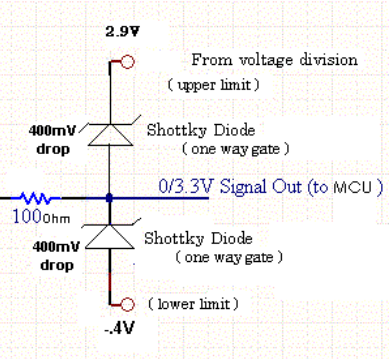
\includegraphics[width=\linewidth]{{images/shottky.png}}
        \caption{Shottky Diode Protection Circuit \cite{b1}}
        \label{fig:shottky}
    \end{figure}
    While Fig. \ref{fig:shottky} recommends values of -0.4V and 2.9V for the
    upper and lower limits, the chosen values of 0V and 3.3V have the same
    precautionary effect. \\ \\
    Finally, opamps were added between each stage of the circuit to allow for
    buffering and separate the voltages of the different subsections. This
    required two opamps in addition to the one used for the gain output. The
    two buffering opamps were not placed with resistors and therefore had no
    amplifying effect on the signal. \\ \\
    The template of this setup is shown in Fig. \ref{fig:template}. \\
    \begin{figure}[h]
        \centering
        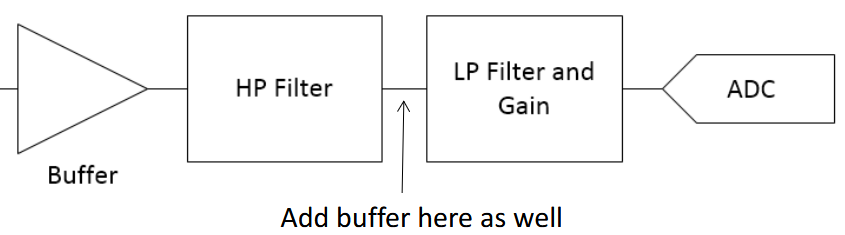
\includegraphics[width=\linewidth]{{images/template.png}}
        \caption{Template of Complete Filtering Circuit}
        \label{fig:template}
    \end{figure}

    Using the values calculated previously with (\ref{eq:cutoff}) and
    (\ref{eq:gain}), the circuit was built in a simulation environment using
    LTSPICE. This completed filtering, amplifying, and protection circuit is
    displayed in Fig. \ref{fig:circuit_sim}. \\
    \begin{figure}[h]
        \centering
        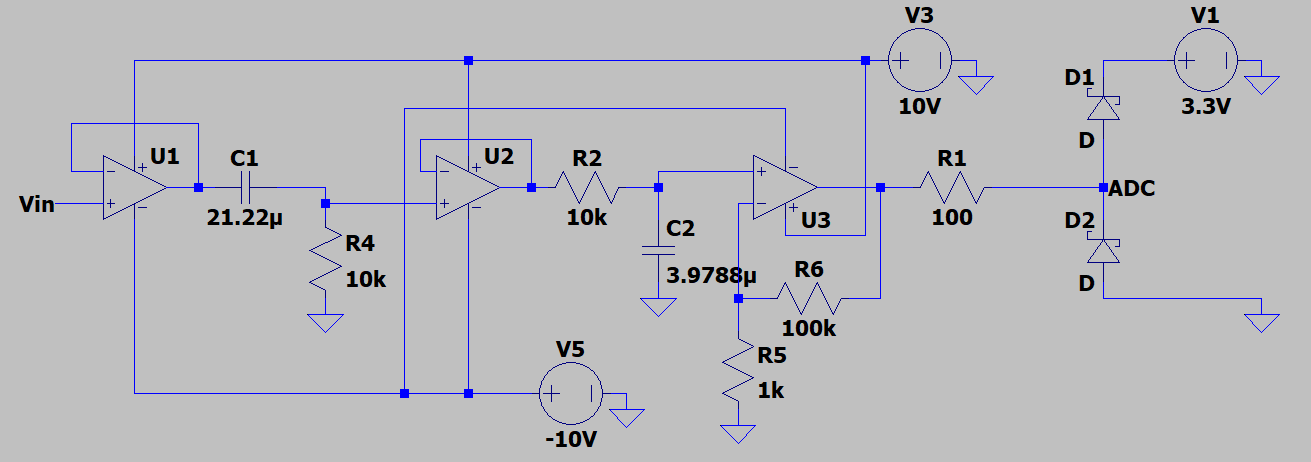
\includegraphics[width=\linewidth]{{images/circuit_sim.png}}
        \caption{Complete Filtering Circuit}
        \label{fig:circuit_sim}
    \end{figure}

    The first iteration of the completed circuit shown in Fig.
    \ref{fig:circuit_sim} was tested twice before being put to use on an actual
    heart rate from a human. First, a simulation was run which used ideal
    values and isn't affected by noise. Secondly, a physical circuit was
    constructed on a breadboard. The setup for this test was identical to how
    the actual sensor would operate with the only difference being the input
    voltage itself. \\ \\
    Instead of connecting to the OPB745 sensor as per the final goal, a
    function generator was used. When set to a frequency of 1Hz, an AC voltage
    of 35mV, and a DC voltage of 500mV, a steady output can be connected to
    the circuit. This is useful for testing as it isolates only the filtering
    section of the circuit and can be used to verify the legitimacy of the
    chosen and calculated values before more complication is introduced with
    the sensing circuitry. \\ \\
    As a consequence of using physical components, there will be some
    variation between the design, what the components chosen claim to be, and
    what the components actually are. This problem was most prevalent for the
    capacitors, but it occured in the resistors as well. \\
    For example, of the two 10k$\Omega$ resistors required, one measured
    9,932$\Omega$ and the other was 10,152$\Omega$. The 100$\Omega$ resistor
    in the protection circuit was measured to be 106$\Omega$. These variations
    had the possibility of causing the most difficulty in the 100k$\Omega$ and
    1k$\Omega$ components used for the gain amplifier. If the values were too
    far off what they claimed, the amplification could be significantly
    altered. Even a 5\% tolerance on each of the resistors creates a possible
    range of approximately 90x to 110x. While this would not be catastrophic
    to the project, such variations are not wanted. \\ \\
    With some searching, however, two resistors were found which were close
    enough to their respective values at 987$\Omega$ and 101,567$\Omega$ to
    keep the gain within reasonable limits at about 103x. \\ \\
    The capacitors were slightly more difficult to source as the designed
    values were not available. To create the 21.22$\mu F$ capacitor, two
    10$\mu F$ components were placed parallel to each other so as to have the
    same effect as one singular component. Because their measured values were
    actually closer to 11$\mu F$ at 10.63$\mu F$ and 10.77$\mu F$, the
    combined capacitance was close the desired amount. \\ \\
    A similar problem existed for the 3.9788$\mu F$ capacitor. In this case,
    two 2$\mu F$ were used with values measuring 1.865$\mu F$ and
    2.193$\mu F$. The constructed circuit is shown in simulation in Fig.
    \ref{fig:circuit_real}. \\
    \begin{figure}[h]
        \centering
        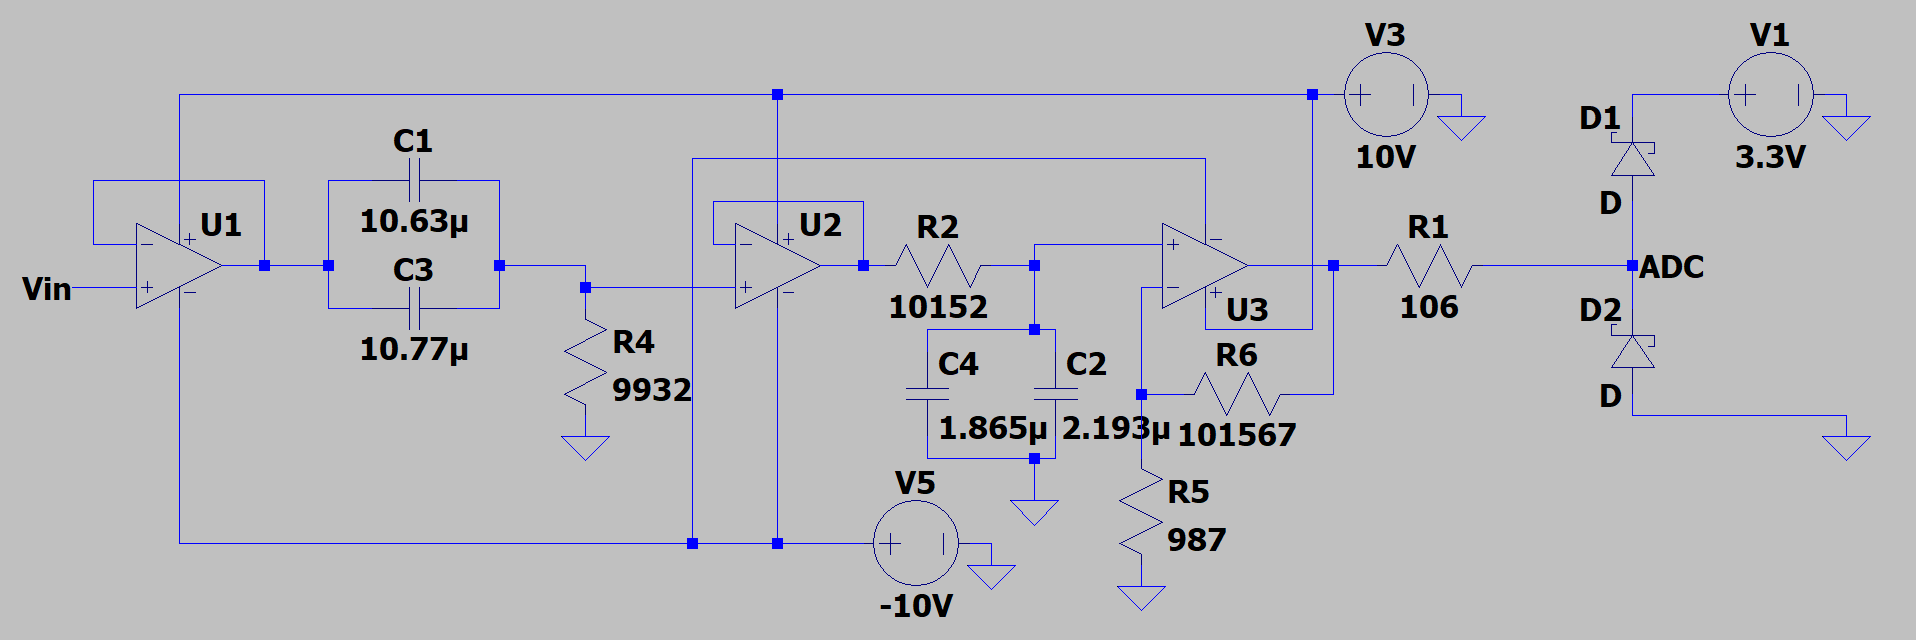
\includegraphics[width=\linewidth]{{images/circuit_real.png}}
        \caption{Complete Filtering Circuit with Measured Values}
        \label{fig:circuit_real}
    \end{figure}

    As a final step for this portion, a C program was written to parse the
    information from the ADC and convert the raw digital values into a useable
    measurement: beats per minute. \\ \\

    --------------------------------------------------------------------------
    EXPLANATION OF HOW THE PROGRAM WORKS
    --------------------------------------------------------------------------

    With the filtering and amplifying setup proven to be accurate, the OPB745
    could be added to the circuit and a real heart rate sensor could be
    constructed. The sensor has a number of ancillary components which are
    laid out in Fig. \ref{fig:opb_setup}. \\
    \begin{figure}[h]
        \centering
        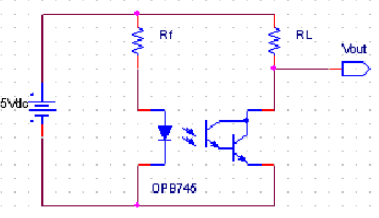
\includegraphics[width=\linewidth]{{images/opb_setup.png}}
        \caption{OPB745 Sensor and Supporting Circuitry \cite{b1}}
        \label{fig:opb_setup}
    \end{figure}
    For the OPB745, two resistors are required. The first, $R_f$ limits the
    current to the LED and protects it from damage. This value is found using
    (\ref{eq:led}).
    \begin{equation}
        R_f = \frac{5V - V_{LED}}{I_f} = \frac{5V - 1.7V}{40mA} = 82.5\Omega
        \label{eq:led}
    \end{equation}
    The values for calculating $R_f$ were found from the OPB745's datasheet
    which denotes a forward voltage across the LED of 1.7V and a maximum
    current before damage at 40mA \cite{b2}. This resulted in a resistance for
    $R_f$ of 82.5$\Omega$, for which a 75$\Omega$ component was used on the
    breadboard. \\ \\ 
    The $R_L$ value is chosen by the designer and was 10k$\Omega$ for this
    case to simplify the number of unique components used. This resistor was
    measured to be 958$\Omega$. \\ \\
    The fully constructed circuit is shown in simulation in Fig.
    \ref{fig:opb_sim} and on the breadboard in Fig. \ref{fig:opb_real}.
    \begin{figure}[h]
        \centering
        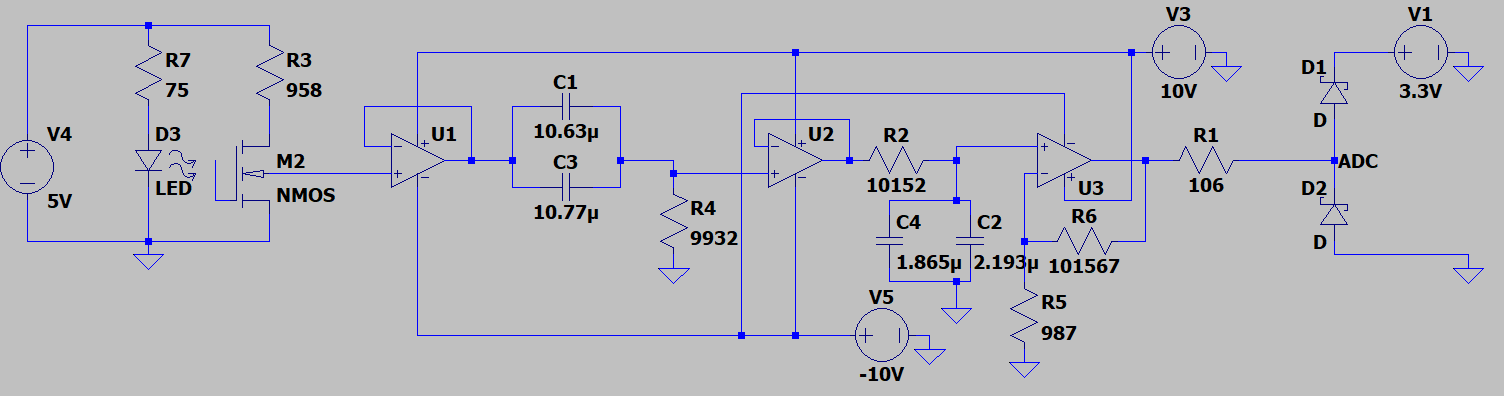
\includegraphics[width=\linewidth]{{images/opb_sim.png}}
        \caption{Full Simulated Circuit with OPB Sensor}
        \label{fig:opb_sim}
    \end{figure}
    \begin{figure}[h]
        \centering
        \includegraphics[width=\linewidth]{{images/opb_real.jpg}}
        \caption{Fully Built Circuit with OPB Sensor}
        \label{fig:opb_real}
    \end{figure}
    
    The final design has a transfer function which is made up of both the low
    pass transfer function shown in (\ref{eq:low_transfer}) and the high pass
    transfer function (\ref{eq:high_transfer}). These two equations are the basic
    form of transfer function equations. What makes this application
    interesting is that they are combined to become a bandpass filter.
    The transfer function for the entire system is the product of
    (\ref{eq:low_transfer}) and (\ref{eq:high_transfer}). \\
    \begin{equation}
        H(j\omega) = \frac{1}{1+j\omega RC}
        \label{eq:low_transfer}
    \end{equation}
    \begin{equation}
        H(j\omega) = \frac{j\omega RC}{1+j\omega RC}
        \label{eq:high_transfer}
    \end{equation}

    The final transfer equation for the entire circuit is
    \ref{eq:full_transfer}. This equation represents the total response of the
    circuit to any input voltage and describes both how the lower values and
    higher values are cut off to form the band which is used for calculations.
    \begin{equation}
        H(j\omega) = \frac{j\omega RC}{2(j\omega RC) + 1 - (\omega RC)^2}
        \label{eq:full_transfer}
    \end{equation}

\section{Results and Analysis}
    At each step in the process of designing, simulations and tests were
    conducted to verify the chosen design constraints. Crucially, the filters
    had to be shown to be working in a simulation before the OPB745 was added.
    This extra component added a lot of variability to the output and
    introduced external factors such as noise, light level, and even how the
    finger was pressed to the sensor which could all significantly warp the
    data. If the filter had an issue which wasn't discovered before testing
    in hardware, the designer could have spent hours trying to debug a problem
    in the wrong part of the circuit. \\ \\
    The simulation was conducted on the complete filtering circuit in LTSPICE
    shown in Fig. \ref{fig:circuit_sim}. An AC sweep was conducted from
    0.1Hz to 10Hz and the result was recorded with a .tran command. The output
    of this test is shown in Fig. \ref{fig:waveform}.
    \begin{figure}[h]
        \centering
        \includegraphics[width=\linewidth]{{images/waveform.png}}
        \caption{Simulated Output of the Circuit with an AC Sweep}
        \label{fig:waveform}
    \end{figure}

    The AC sweep demonstrates possible inputs to the circuit and can be used
    to gauge how it will react to the OPB sensor. Shown in the middle of Fig.
    \ref{fig:waveform} is the inputted values. This line is nearly flat and
    any variations are difficult to perceive with the naked eye. The much
    larger, sweeping waveforms are the amplified output. This is what the ADC
    will receive from the filter. It is clear that the amplified signal will
    be significantly easier to parse and detect changes in. Rather than
    fluctuating slightly around a set voltage, the signal spikes and drops at
    a regular interval. \\ \\ 
    The output of the simulation in Fig. \ref{fig:waveform} confirmed the
    correct design of the filtering circuit, but its construction had to also
    be tested. This was done on a breadboard with the function generator
    replacing the AC sweep command. The output was recorded via an
    oscilloscope. This is shown in Fig. \ref{fig:1hz_scope}. \\
    \begin{figure}[h]
        \centering
        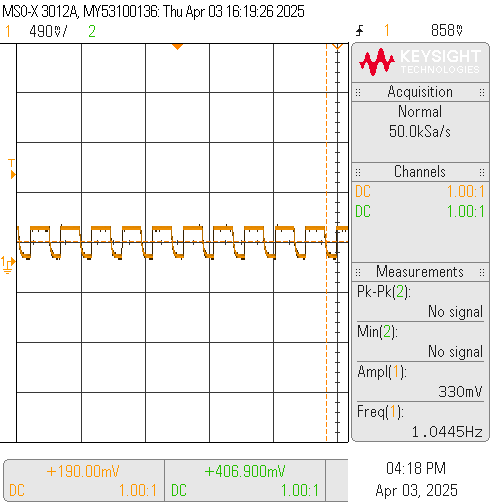
\includegraphics[width=\linewidth]{{images/1hz_scope.png}}
        \caption{Oscilloscope Capture of the Function Generator at 1Hz}
        \label{fig:1hz_scope}
    \end{figure}
    The waveform captured peaks exactly every one second. This is picked up by
    the constructed circuit. What is important to note is that there is no
    gradual ramp up or down for the voltage. It spikes, holds, and then drops.
    This is due to the filters implemented in the signal conditioning stage
    which remove all of the voltages not at the extremes. \\ \\

    The code was also tested at this point as checking the functionality was
    easy. Because the function generator was set at 1Hz, the PuTTY terminal
    should show exactly 60 BPM. This is almost exactly what happened, captured
    in Fig. \ref{fig:1hz_putty}. \\
    \begin{figure}[h]
        \centering
        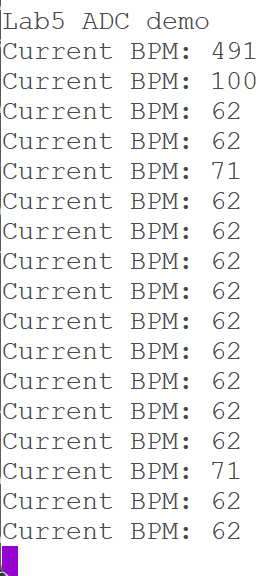
\includegraphics[width=150pt]{{images/1hz_putty.png}}
        \caption{Capture of the PuTTY Output Terminal at 1Hz}
        \label{fig:1hz_putty}
    \end{figure}
    While there was some settling that occurred at the start and occasional
    blimps up to 71 BPM, the program consistently output 62 BPM which is
    within a reasonable margin of error of the expected value. \\ \\

    It was important to ensure, however, that the program was not tuned only
    for 1Hz and that it could operate properly at other frequencies as well.
    To evaluate this, the function generator was set to 800mHz and the same
    test was conducted. The oscilloscope and PuTTY outputs are shown in Fig.
    \ref{fig:800mhz_scope} and \ref{fig:800mhz_putty}
    \begin{figure}[h]
        \centering
        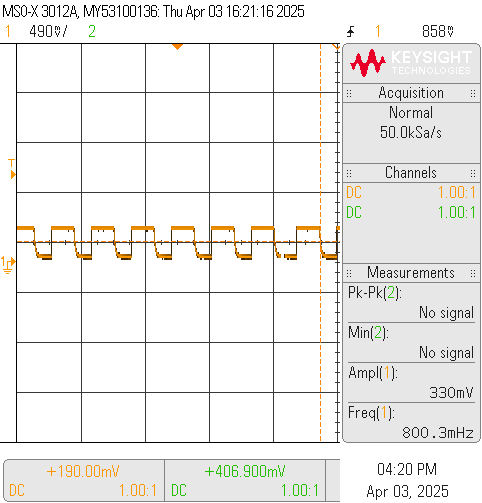
\includegraphics[width=\linewidth]{{images/800mhz_scope.png}}
        \caption{Oscilloscope Capture of the Function Generator at 800mHz}
        \label{fig:800mhz_scope}
    \end{figure}
    \begin{figure}[h]
        \centering
        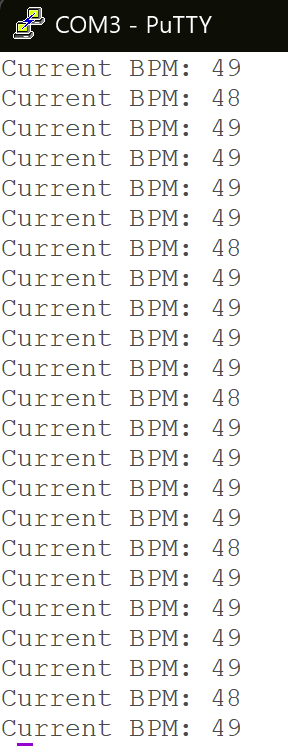
\includegraphics[width=150pt]{{images/800mhz_putty.png}}
        \caption{Capture of the PuTTY Output Terminal at 800mHz}
        \label{fig:800mhz_putty}
    \end{figure}
    Because the output shown in Fig. \ref{fig:800mhz_putty} is exactly as
    expected: 80\% lower than at 1Hz; the code can be verified to be correct.
    \\ \\

    With the circuit construction and the code both tested, the last step was
    to actually construct the heart rate sensor and test whether the filter
    worked properly. This is where some problems arose. When the OPB745 was
    attached to the input of the circuit in place of the function generator,
    no changes in output were visible on the oscilloscope or in the PuTTY
    terminal. \\ \\
    It was determined via probing different points along the conditioning that
    the output voltage of the OPB was changing by such minute amounts that it
    was imperceptible to the oscilloscope or ADC, despite the gain implemented
    in the filter. It was necessary, therefore, to increase the gain into the
    filtering circuit before either of the filters. This was achieved with
    another opamp and two resistors. \\ \\

    The final output of this circuit, tested with a human finger pressed
    against the OPB745 is shown in Fig. \ref{fig:heartrate_scope}.
    \begin{figure}[h]
        \centering
        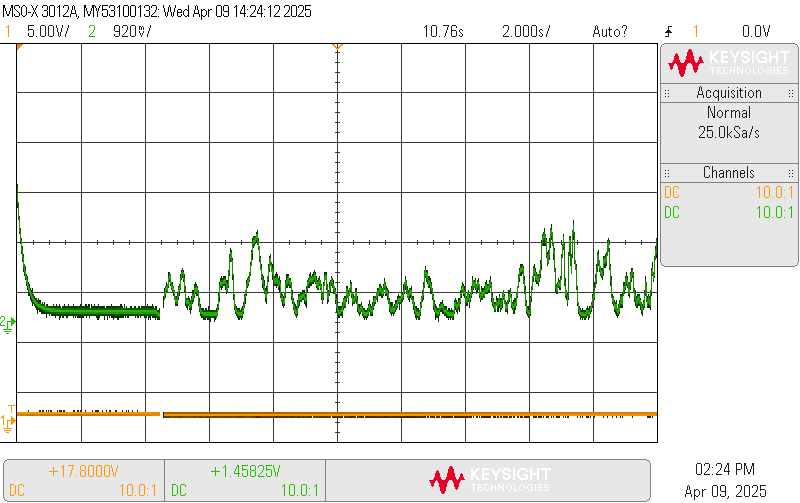
\includegraphics[width=\linewidth]{{images/heartrate_scope.png}}
        \caption{Oscilloscope Capture of the Heart Rate Sensor}
        \label{fig:heartrate_scope}
    \end{figure}

\section{Conclusion}
    The ultimate goal of this project was to design, simulate, and build a
    circuit which could measure the very small change in light reflected off a
    human bone as a result of changes in blood pressure to determine that
    person's heart rate. Using a combination of amplifiers, filters, and
    protection circuits, this goal was achieved. Along each step of the
    process, tests were conducted which would make troubleshooting later on
    much more straightforward as any issues could be attributed to the section
    being worked on presently. While there were some challenges along the way,
    this strategy meant that they were quickly discovered and remedied. The
    heart rate sensor worked as expected and though likely not accurate enough
    for real medical applications, was a functional device which could measure
    and calculate BPM.

\begin{thebibliography}{00}
    \bibitem{b1} S. Soldavini, \"IDE\_Manual\_2025S\", Apr 2025.
    \bibitem{b2} OPTEK, Reflective Object Sensor Type OPB745, June 1996
    \end{thebibliography}

\end{document}
